%%%%%%%%%%%%%%%%%%%%%%%%%%%%%%%%%%%%%%%%%%%%%%%%%%%%%%%%%%%%%%%
%% BRIEF VERSION OF OXFORD THESIS TEMPLATE FOR CHAPTER PREVIEWS

%%%%% CHOOSE PAGE LAYOUT
% format for PDF output (ie equal margins, no extra blank pages):
\documentclass[a4paper,nobind]{templates/ociamthesis}

% UL 5 January 2021 - add packages used by kableExtra
\usepackage{booktabs}
\usepackage{longtable}
\usepackage{array}
\usepackage{multirow}
\usepackage{wrapfig}
\usepackage{colortbl}
\usepackage{pdflscape}
\usepackage{tabu}
\usepackage{threeparttable}
\usepackage{threeparttablex}
\usepackage[normalem]{ulem}
\usepackage{makecell}
\usepackage[colorlinks=false,pdfpagelabels,hidelinks=]{hyperref}
\usepackage{float}


%UL set section header spacing
\usepackage{titlesec}
% 
\titlespacing\subsubsection{0pt}{24pt plus 4pt minus 2pt}{0pt plus 2pt minus 2pt}

% UL 30 Nov 2018 pandoc puts lists in 'tightlist' command when no space between bullet points in Rmd file
\providecommand{\tightlist}{%
  \setlength{\itemsep}{0pt}\setlength{\parskip}{0pt}}
 
% UL 1 Dec 2018, fix to include code in shaded environments
\usepackage{color}
\usepackage{fancyvrb}
\newcommand{\VerbBar}{|}
\newcommand{\VERB}{\Verb[commandchars=\\\{\}]}
\DefineVerbatimEnvironment{Highlighting}{Verbatim}{commandchars=\\\{\}}
% Add ',fontsize=\small' for more characters per line
\usepackage{framed}
\definecolor{shadecolor}{RGB}{248,248,248}
\newenvironment{Shaded}{\begin{snugshade}}{\end{snugshade}}
\newcommand{\AlertTok}[1]{\textcolor[rgb]{0.94,0.16,0.16}{#1}}
\newcommand{\AnnotationTok}[1]{\textcolor[rgb]{0.56,0.35,0.01}{\textbf{\textit{#1}}}}
\newcommand{\AttributeTok}[1]{\textcolor[rgb]{0.77,0.63,0.00}{#1}}
\newcommand{\BaseNTok}[1]{\textcolor[rgb]{0.00,0.00,0.81}{#1}}
\newcommand{\BuiltInTok}[1]{#1}
\newcommand{\CharTok}[1]{\textcolor[rgb]{0.31,0.60,0.02}{#1}}
\newcommand{\CommentTok}[1]{\textcolor[rgb]{0.56,0.35,0.01}{\textit{#1}}}
\newcommand{\CommentVarTok}[1]{\textcolor[rgb]{0.56,0.35,0.01}{\textbf{\textit{#1}}}}
\newcommand{\ConstantTok}[1]{\textcolor[rgb]{0.00,0.00,0.00}{#1}}
\newcommand{\ControlFlowTok}[1]{\textcolor[rgb]{0.13,0.29,0.53}{\textbf{#1}}}
\newcommand{\DataTypeTok}[1]{\textcolor[rgb]{0.13,0.29,0.53}{#1}}
\newcommand{\DecValTok}[1]{\textcolor[rgb]{0.00,0.00,0.81}{#1}}
\newcommand{\DocumentationTok}[1]{\textcolor[rgb]{0.56,0.35,0.01}{\textbf{\textit{#1}}}}
\newcommand{\ErrorTok}[1]{\textcolor[rgb]{0.64,0.00,0.00}{\textbf{#1}}}
\newcommand{\ExtensionTok}[1]{#1}
\newcommand{\FloatTok}[1]{\textcolor[rgb]{0.00,0.00,0.81}{#1}}
\newcommand{\FunctionTok}[1]{\textcolor[rgb]{0.00,0.00,0.00}{#1}}
\newcommand{\ImportTok}[1]{#1}
\newcommand{\InformationTok}[1]{\textcolor[rgb]{0.56,0.35,0.01}{\textbf{\textit{#1}}}}
\newcommand{\KeywordTok}[1]{\textcolor[rgb]{0.13,0.29,0.53}{\textbf{#1}}}
\newcommand{\NormalTok}[1]{#1}
\newcommand{\OperatorTok}[1]{\textcolor[rgb]{0.81,0.36,0.00}{\textbf{#1}}}
\newcommand{\OtherTok}[1]{\textcolor[rgb]{0.56,0.35,0.01}{#1}}
\newcommand{\PreprocessorTok}[1]{\textcolor[rgb]{0.56,0.35,0.01}{\textit{#1}}}
\newcommand{\RegionMarkerTok}[1]{#1}
\newcommand{\SpecialCharTok}[1]{\textcolor[rgb]{0.00,0.00,0.00}{#1}}
\newcommand{\SpecialStringTok}[1]{\textcolor[rgb]{0.31,0.60,0.02}{#1}}
\newcommand{\StringTok}[1]{\textcolor[rgb]{0.31,0.60,0.02}{#1}}
\newcommand{\VariableTok}[1]{\textcolor[rgb]{0.00,0.00,0.00}{#1}}
\newcommand{\VerbatimStringTok}[1]{\textcolor[rgb]{0.31,0.60,0.02}{#1}}
\newcommand{\WarningTok}[1]{\textcolor[rgb]{0.56,0.35,0.01}{\textbf{\textit{#1}}}}

%UL 2 Dec 2018 add a bit of white space before and after code blocks
\renewenvironment{Shaded}
{
  \vspace{10pt}%
  \begin{snugshade}%
}{%
  \end{snugshade}%
  \vspace{8pt}%
}
%UL 2 Dec 2018 reduce whitespace around verbatim environments
\usepackage{etoolbox}
\makeatletter
\preto{\@verbatim}{\topsep=0pt \partopsep=0pt }
\makeatother

%UL 28 Mar 2019, enable strikethrough
\usepackage[normalem]{ulem}

%UL use soul package for correction highlighting
\usepackage{soul}
\usepackage{xcolor}
\newcommand{\ctext}[3][RGB]{%
  \begingroup
  \definecolor{hlcolor}{#1}{#2}\sethlcolor{hlcolor}%
  \hl{#3}%
  \endgroup
}
\soulregister\ref7
\soulregister\cite7
\soulregister\autocite7
\soulregister\textcite7
\soulregister\pageref7

%UL 3 Nov 2019, avoid mysterious error from not having hyperref included
\usepackage{hyperref}

%%%%% SELECT YOUR DRAFT OPTIONS
% Three options going on here; use in any combination.  But remember to turn the first two off before
% generating a PDF to send to the printer!

% This adds a "DRAFT" footer to every normal page.  (The first page of each chapter is not a "normal" page.)

% This highlights (in blue) corrections marked with (for words) \mccorrect{blah} or (for whole
% paragraphs) \begin{mccorrection} . . . \end{mccorrection}.  This can be useful for sending a PDF of
% your corrected thesis to your examiners for review.  Turn it off, and the blue disappears.

%%%%% BIBLIOGRAPHY SETUP
% Note that your bibliography will require some tweaking depending on your department, preferred format, etc.
% The options included below are just very basic "sciencey" and "humanitiesey" options to get started.
% If you've not used LaTeX before, I recommend reading a little about biblatex/biber and getting started with it.
% If you're already a LaTeX pro and are used to natbib or something, modify as necessary.
% Either way, you'll have to choose and configure an appropriate bibliography format...

% The science-type option: numerical in-text citation with references in order of appearance.
% \usepackage[style=numeric-comp, sorting=none, backend=biber, doi=false, isbn=false]{biblatex}
% \newcommand*{\bibtitle}{References}

% The humanities-type option: author-year in-text citation with an alphabetical works cited.
% \usepackage[style=authoryear, sorting=nyt, backend=biber, maxcitenames=2, useprefix, doi=false, isbn=false]{biblatex}
% \newcommand*{\bibtitle}{Works Cited}

%UL 3 Dec 2018: set this from YAML in index.Rmd
\usepackage[style=numeric-comp, sorting=none, backend=biber, doi=false, isbn=false]{biblatex}
\newcommand*{\bibtitle}{References}

% This makes the bibliography left-aligned (not 'justified') and slightly smaller font.
\renewcommand*{\bibfont}{\raggedright\small}

% Change this to the name of your .bib file (usually exported from a citation manager like Zotero or EndNote).
\addbibresource{references.bib}

%%%%% YOUR OWN PERSONAL MACROS
% This is a good place to dump your own LaTeX macros as they come up.

% To make text superscripts shortcuts
	\renewcommand{\th}{\textsuperscript{th}} % ex: I won 4\th place
	\newcommand{\nd}{\textsuperscript{nd}}
	\renewcommand{\st}{\textsuperscript{st}}
	\newcommand{\rd}{\textsuperscript{rd}}

%%%%% THE ACTUAL DOCUMENT STARTS HERE
\begin{document}

%%%%% CHOOSE YOUR LINE SPACING HERE
% This is the official option.  Use it for your submission copy and library copy:
\setlength{\textbaselineskip}{22pt plus2pt}
% This is closer spacing (about 1.5-spaced) that you might prefer for your personal copies:
%\setlength{\textbaselineskip}{18pt plus2pt minus1pt}

% UL: You can set the general paragraph spacing here - I've set it to 2pt (was 0) so
% it's less claustrophobic
\setlength{\parskip}{2pt plus 1pt}

% Leave this line alone; it gets things started for the real document.
\setlength{\baselineskip}{\textbaselineskip}

% all your chapters and appendices will appear here
\hypertarget{dat-and-meth}{%
\chapter{Data and methodology}\label{dat-and-meth}}

\chaptermark{Data and methodology}

\minitoc 

\hypertarget{data}{%
\section{Data}\label{data}}

\noindent We worked with daily returns on the EURO STOXX 50 Index denoted in EUR from 31 dicembre, 1986 to 27 aprile, 2021. It is the leading blue-chip index of the Eurozone, was founded in 1999 and covers 50 of the most liquid and largest (in terms of free-float market capitalization) stocks. Its composition is reviewed annually in September, from each of the 19 EURO STOXX Supersector indices the biggest stocks are selected until the coverage is at 60\% of the free-float market cap of each of the EURO STOXX Supersector index then all the current EURO STOXX 50 stocks are used in the selection list from which the largest 40 in terms of free-float market cap are selected and the remaining 10 stocks are chosen among those ranked between 41 and 60 \autocite{EUROSTOXXFactSheet}.

\noindent The calculation of the index is made with the @ref(eq:Laspeyres.formula), that measures the changes in price of the index for fixed weights.

\begin{align}
\text { Index }_{t}=\frac{\sum_{i=1}^{n}\left(p_{i t} \cdot s_{i t} \cdot f f_{i t} \cdot c f_{i t} \cdot x_{i t}\right)}{D_{t}}=\frac{M_{t}}{D_{t}}
(\#eq:Laspeyres.formula)
\end{align}

\noindent where: t = Time the index is computed \(n\) = Number of companies in the index \(p_{i t}\) = Price of company (\(i\)) at time (t) \(s_{i t}\) = Number of shares of company (\(i\)) at time (t) \(f f_{i t}\) = Free float factor of company (\(i\)) at time (t) \(c f_{i t}\) = Weighting cap factor of company (\(i\)) at time (t) \(x_{i t}\) = Exchange rate from local currency into index currency for company (\(i\)) at time (t) \(M_{t}\) = Free-float market capitalization of the index at time (t) \(D_{t}\) = Divisor of the index at time (t)

\noindent Changes in weights caused by corporate actions are proportionally distributed across the components of the index and the index Divisor is computed with the @ref(eq:Price.weighted) formula.

\begin{align}
D_{t+1}=D_{t} \cdot \frac{\sum_{i=1}^{n}\left(p_{i t} \cdot s_{i t} \cdot f f_{i t} \cdot c f_{i t} \cdot x_{i t}\right) \pm \Delta M C_{t+1}}{\sum_{i=1}^{n}\left(p_{i t} \cdot s_{i t} \cdot f f_{i t} \cdot c f_{i t} \cdot x_{i t}\right)}
(\#eq:Price.weighted)
\end{align}

\noindent where: \noindent \(\Delta M C_{t+1}\) = Difference between the closing market capitalization of the index and the adjusted closing market capitalization of the index

(Optional)

The same analysis has been performed for the INDEX 1, INDEX 2, INDEX 3 and the INDEX 4 indexes with not qualitatively different conclusions(\ldots.hopefully\ldots.). The findings of these researches are available upon requests.

\newpage

\hypertarget{descriptives}{%
\subsection{Descriptives}\label{descriptives}}

\hypertarget{table-of-summary-statistics}{%
\subsubsection{Table of summary statistics}\label{table-of-summary-statistics}}

Equation \ref{tab:dsTable} provides the main statistics describing the return series analyzed. Returns are computed with equation @ref(eq:log.returns) formula

\begin{align}
R_{t}=100\left(\ln \left(I_{t}\right)-\ln \left(I_{t-1}\right)\right)
  (\#eq:log.returns)
\end{align}

\noindent Where \(I_{t}\) is the index price at time \(t\) and \(I_{t-1}\) is the index price at \(t-1\).

\noindent The Arithmetic Mean of the series is 0.017\% with a standard deviation of 1.307\% and a median of 0.036 which translate to an annualized mean of 4.208\% and an annualized standard deviation of 20.748\%. The Skewness statistic is highly significant and negative at -0.31 and the excess Kurtosis is also highly significant and positive at 7.208. These 2 statistics give an overview of the distribution of the returns which has thicker tails than the normal distribution with a higher presence of left tail observations. A formal test such as the Jarque-Bera one with its statistic at 19528.62 and a high statistical significance, confirms the non normality feeling given by the Skewness and Kurtosis.

\noindent The right column of @ref:stats displays the same descriptives but for the standardizes residuals obtained from a simple GARCH model as mentioned in @ref:stats in Note 2\(*\). Again, Skewness statistic at -0.633 with a high statistical significance level and the excess Kurtosis at 5.134 also with a high statistical significance, suggest a non normal distribution of the standardized residuals and the Jarque-Bera statistic at NA, given its high significance, confirms the rejection of the normality assumption.

\begin{table}[h!]

\caption{\label{tab:dsTable}Summary statistics of the returns}
\centering
\begin{threeparttable}
\begin{tabular}[t]{lll}
\toprule
Statistics & Eurostoxx.50 & Standardized.Residuals\\
\midrule
Arithmetic Mean & 0.0167 & -0.0409\\
Median & 0.0357 & -0.0193\\
Maximum & 10.4376 & 5.7126\\
Minimum & -13.2404 & -11.7732\\
Stdev & 1.307 & 0.9992\\
\addlinespace
Skewness & -0.31 & -0.6327\\
 & (0***) & (0***)\\
Excess Kurtosis & 7.2083 & 5.134\\
 & (0***) & (0***)\\
Jarque-Bera & 19528.6196*** & 10431.0514***\\
\bottomrule
\end{tabular}
\begin{tablenotes}
\item makecell[l]{\ 1): This table shows the descriptive statistics of the daily percentage returns of               over the period 1987-01-01 to 2021-04-27 (8954 observations). Including arithmetic mean, median, maximum, minimum, standard deviation, skewness, excess kurtosis and the Jarque-Bera test.}
\item makecell[c]{2): The standardized residual is derived from a maximum likelyhood estimation (simple GARCH model) as follows: \}
\item \$R\_t=\textbackslash{}alpha\_0+\textbackslash{}alpha\_1 R\_\{t-1\}+z\_t \textbackslash{}sigma\_t\$
\item \$\textbackslash{}sigma\_t\textasciicircum{}2=\textbackslash{}beta\_0+\textbackslash{}beta\_1 \textbackslash{}sigma\_\{t-1\}\textasciicircum{}2 z\_\{t-1\}\textasciicircum{}2+\textbackslash{}beta\_2 \textbackslash{}sigma\_\{t-1\}\textasciicircum{}2,\$
\item Where \$z\$ is the standard residual (assumed to have a normal distribution)
\item  3): \$*\$, \$**\$, \$***\$ represent significance levels at the 5\%, 1\% and <1\%
\end{tablenotes}
\end{threeparttable}
\end{table}

\newpage

\hypertarget{descriptive-figures}{%
\subsubsection{Descriptive figures}\label{descriptive-figures}}

\hypertarget{stylized-facts}{%
\paragraph{Stylized facts}\label{stylized-facts}}

As can be seen in figure \ref{fig:plot1} the Euro area equity and later, since 1999 the EuroStoxx 50 went up during the tech (``dot com'') bubble reaching an ATH of €5464.43. Then, there was a correction to boom again until the burst of the 2008 financial crisis. After which it decreased significantly. With an ATL at 09 marzo, 2009 of €1809.98. There is an improvement, but then the European debt crisis, with it's peak in 2010-2012, occurred. From then there was some improvement until the ``health crisis'', which arrived in Europe, February 2020. This crisis recovered very quickly reaching already values higher then the pre-COVID crisis level.

\begin{figure}[h]

{\centering 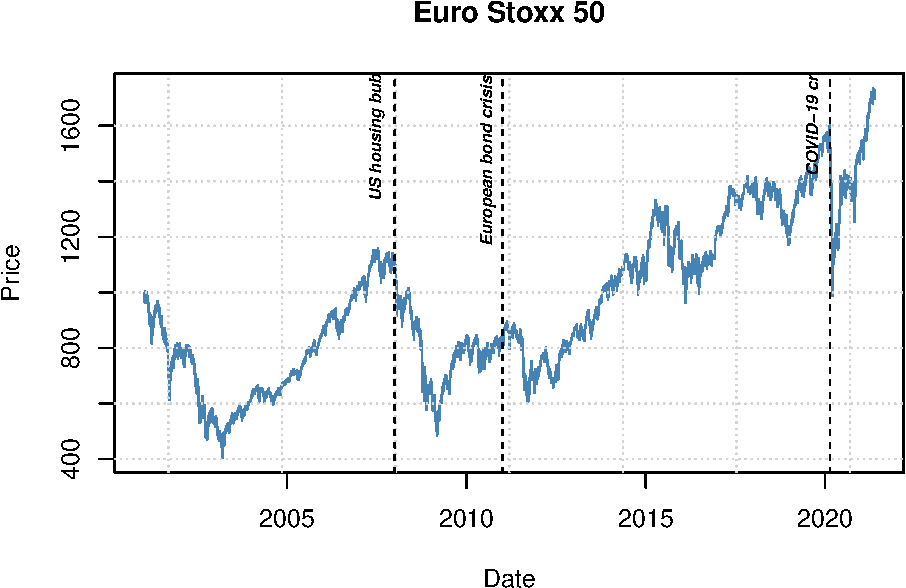
\includegraphics[width=1\linewidth]{03-Data-meth_files/figure-latex/plot1-1} 

}

\caption{Eurostoxx 50 Price Index prices}\label{fig:plot1}
\end{figure}

\newpage

In figure \ref{fig:plot2} the daily log-returns are visualized. A stylized fact that is observable is the volatility clustering. As can be seen: periods of large volatility are mostly followed by large volatility and small volatility by small volatility.

\begin{figure}[h]

{\centering 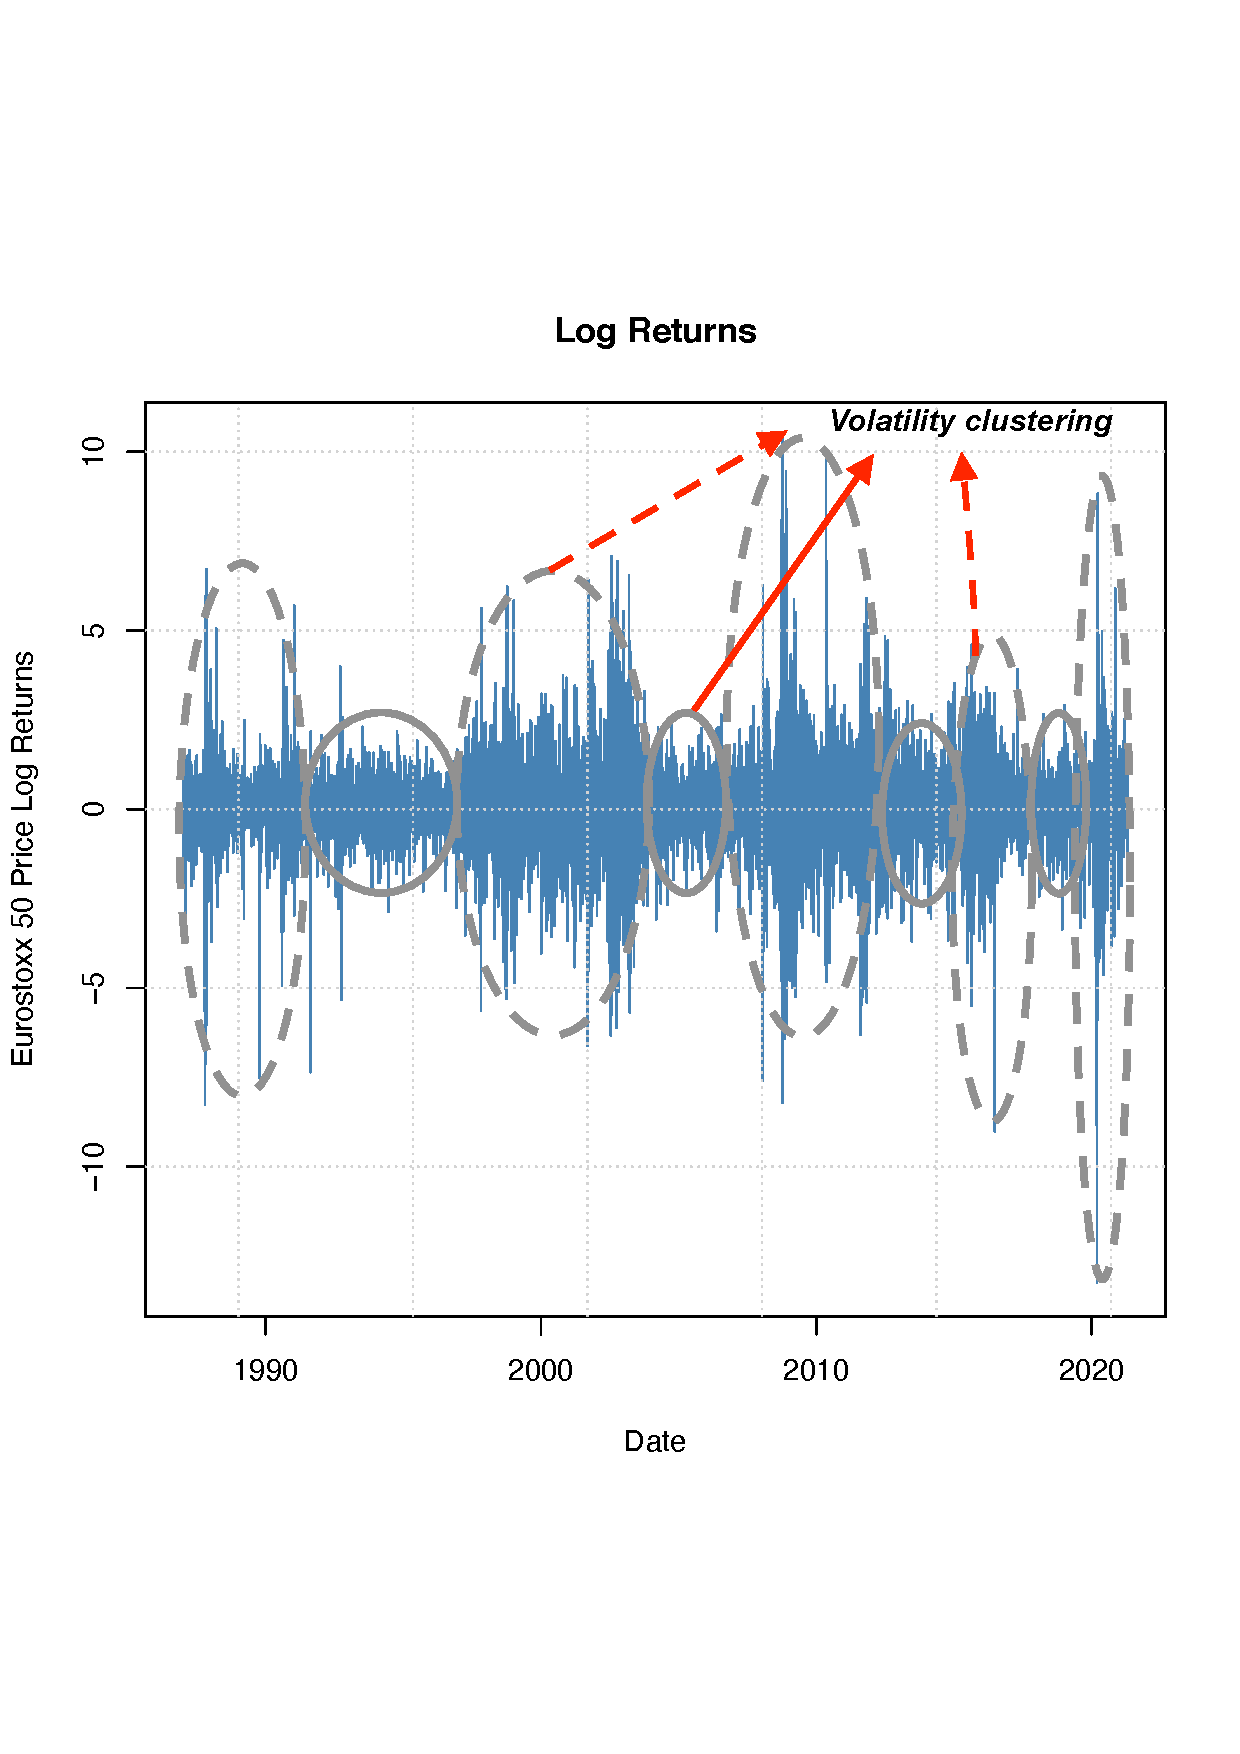
\includegraphics[width=0.75\linewidth]{figures/vol-clustering-final-withcircles} 

}

\caption{Eurostoxx 50 Price Index log returns}\label{fig:plot2}
\end{figure}

\begin{figure}[h]

{\centering 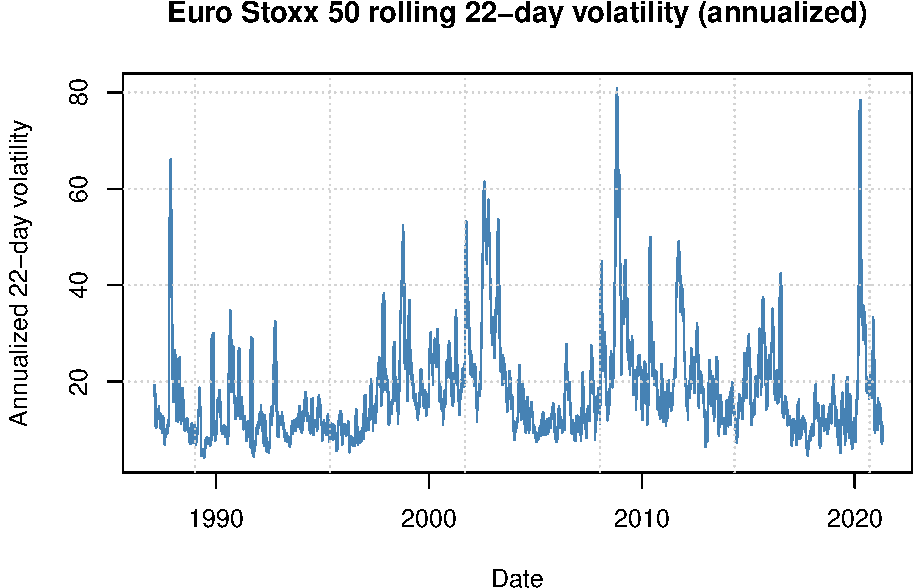
\includegraphics[width=0.75\linewidth]{03-Data-meth_files/figure-latex/plot3-1} 

}

\caption{Eurostoxx 50 rolling volatility (22 days, calculated over 252 days)}\label{fig:plot3}
\end{figure}

\newpage

In figure \ref{fig:plot4} the density distribution of the log returns are examined. As can be seen, as already mentioned in part \ref{styl-facts}, log returns are not really normally distributed. So

\begin{figure}

{\centering 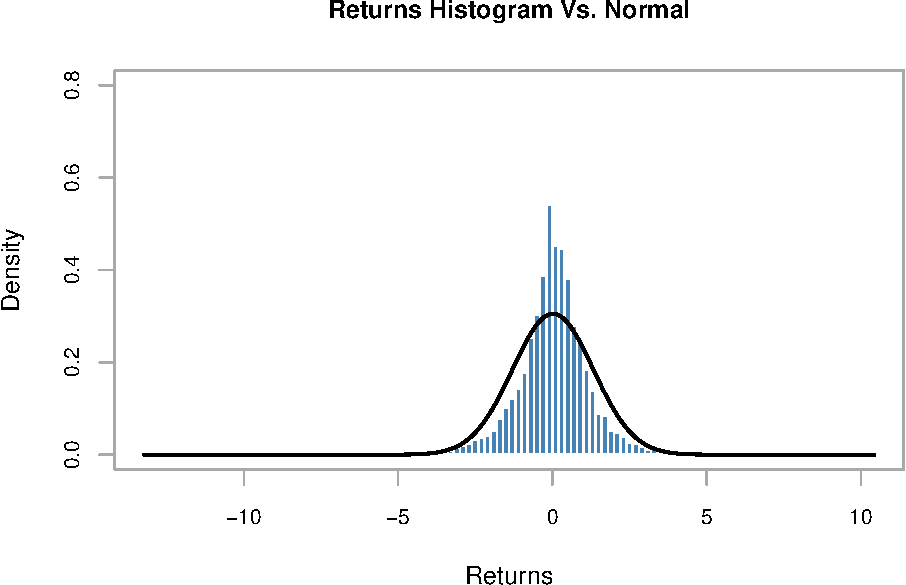
\includegraphics[width=0.75\linewidth]{03-Data-meth_files/figure-latex/plot4-1} 

}

\caption{Density vs. Normal Eurostoxx 50 log returns)}\label{fig:plot4}
\end{figure}

\newpage

*

heteroscedasticity* As can be seen

\begin{figure}[h]

{\centering 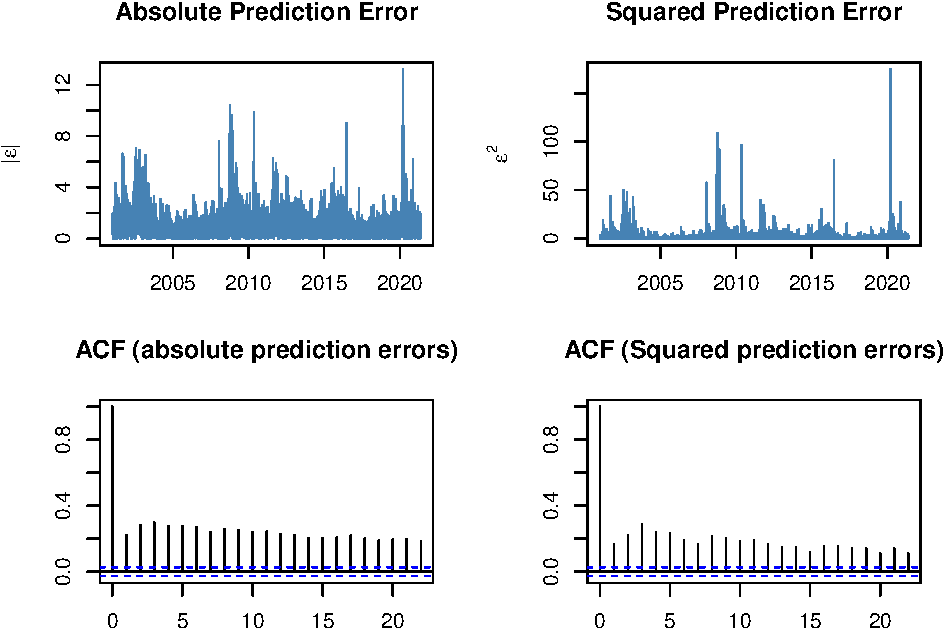
\includegraphics[width=0.75\linewidth]{03-Data-meth_files/figure-latex/acfplots-1} 

}

\caption{Absolute prediction errors}\label{fig:acfplots}
\end{figure}

\clearpage

\hypertarget{methodology}{%
\section{Methodology}\label{methodology}}

\hypertarget{garch-models}{%
\subsection{Garch models}\label{garch-models}}

As already mentioned in \ldots, GARCH models GARCH, EGARCH, IGARCH, GJRGARCH, NGARCH, TGARCH and NAGARCH (or TSGARCH) will be estimated. Additionally the distributions will be examined as well, including the normal, student-t distribution, skewed student-t distribution, generalized error distribution, skewed generalized error distribution and the skewed generalized t distribution.

They will be estimated using maximum likelihood. As already mentioned, fortunately, Alexios \textcite{alexios2020} has made it easy for us to implement this methodology in the R language (v.3.6.1) with the package ``rugarch'' v.1.4-4 (\emph{R univariate garch}), which gives us a bit more time to focus on the results and the interpretation.

Maximum likelihood estimation is a method to find the distribution parameters that best fit the observed data, through maximization of the likelihood function, or the computationally more efficient log-likelihood function (by taking the natural logarithm). It is assumed that the return data is i.i.d. and that there is some underlying parametrized density function \(f\) with one or more parameters that generate the data, defined as a vector \(\theta\) (\eqref{eq:pdf}). These functions are based on the joint probability distribution of the observed data (equation \eqref{eq:logl}). Subsequently, the (log)likelihood function is maximized using an optimization algorithm (equation \eqref{eq:optim}).

\begin{align} 
  y_1,y_2,...,y_N \sim i.i.d
    \\
  y_i \sim f(y|\theta)
 \label{eq:pdf}
\end{align}

\begin{align} 
 L(\theta) = \prod^N_{i=1}f(y_i|\theta)
  \\
 \log(L(\theta)) = \sum^N_{i=1} \log f(y_i |\theta)
 \label{eq:logl}
\end{align}

\begin{align} 
\theta^{*} = arg \max_{\theta} [ L] \\
\theta^{*} = arg \max_{\theta} [\log(L)]
 \label{eq:optim}
\end{align}

\hypertarget{acd-models-meth}{%
\subsection{ACD models}\label{acd-models-meth}}

Following \textcite{ghalanos2016}, arguments of ACD models are specified as in \textcite{hansen1994}. The density function \(f(y|\alpha)\) has parameters \(\alpha_t = (\mu_t, \sigma_t, \nu_t)\), with equation \eqref{eq:cmean}, the conditional mean equation. Equation \eqref{eq:cvariance} as the conditional variance. And \(\nu_t=\nu(\theta,x_t)\) the remaining parameters of the distribution like the skewness and kurtosis (shape) parameters.

\begin{align} 
\mu_{t}=\mu\left(\theta, x_{t}\right)=E\left(y_{t} \mid x_{t}\right)
 \label{eq:cmean}
\end{align}

\begin{align}
\sigma_{t}^{2}=\sigma^{2}\left(\theta, x_{t}\right)=E\left(\left(y_{t}-\mu_{t}^{2}\right) \mid x_{t}\right)
 \label{eq:cvariance}
\end{align}

To further explain the difference between GARCH and ACD. The scaled innovations are given by equation \eqref{eq:scaledinn}. The conditional density is given by equation \eqref{eq:conddens} and related to the density function \(f(y|\alpha)\) as in equation \eqref{eq:densityconddens}.

\begin{align}
z_{t}(\theta)=\frac{y_{t}-\mu\left(\theta, x_{t}\right)}{\sigma\left(\theta, x_{t}\right)}
\label{eq:scaledinn}
\end{align}

\begin{align}
g\left(z \mid \eta_{t}\right)=\frac{d}{d z} P\left(z_{t}<z \mid \eta_{t}\right)
\label{eq:conddens}
\end{align}

\begin{align}
f\left(y_{t} \mid \mu_{t}, \sigma_{t}^{2}, \eta_{t}\right)=\frac{1}{\sigma_{t}} g\left(z_{t} \mid \eta_{t}\right)
\end{align}
\label{eq:densityconddens}

Again \textcite{ghalanos2016} makes it easier to implement the somewhat complex ACD models using the R language with package ``racd''.

\hypertarget{control-tests}{%
\subsection{Control Tests}\label{control-tests}}

\hypertarget{unconditional-coverage-test-of-kupiec1995}{%
\subsubsection{\texorpdfstring{Unconditional coverage test of \textcite{kupiec1995}}{Unconditional coverage test of @kupiec1995}}\label{unconditional-coverage-test-of-kupiec1995}}

A number of tests are computed to see if the value-at-risk estimations capture the actual losses well. A first one is the unconditional coverage test by \textcite{kupiec1995}. The unconditional coverage or proportion of failures method tests if the actual value-at-risk exceedances are consistent with the expected exceedances (a chosen percentile, e.g.~1\% percentile) of the VaR model. Following \textcite{kupiec1995} and \textcite{ghalanos2020}, the number of exceedence follow a binomial distribution (with thus probability equal to the significance level or expected proportion) under the null hypothesis of a correct VaR model. The test is conducted as a likelihood ratio test with statistic like in equation \eqref{eq:uccov}, with \(p\) the probability of an exceedence for a confidence level, \(N\) the sample size and \(X\) the number of exceedence. The null hypothesis states that the test statistic \(L R^{u c}\) is \(\chi^2\)-distributed with one degree of freedom or that the probability of failure \(\hat p\) is equal to the chosen percentile \(\alpha\).

\begin{align}
L R^{u c}=-2 \ln \left(\frac{(1-p)^{N-X} p^{X}}{\left(1-\frac{X}{N}\right)^{N-X}\left(\frac{X}{N}\right)^{X}}\right)
\label{eq:uccov}
\end{align}

\hypertarget{conditional-coverage-test-of-christoffersen2001}{%
\subsubsection{\texorpdfstring{Conditional coverage test of \textcite{christoffersen2001}}{Conditional coverage test of @christoffersen2001}}\label{conditional-coverage-test-of-christoffersen2001}}

\textcite{christoffersen2001} proposed the conditional coverage test. It is tests for unconditional covrage and serial independence. The serial independence is important while the \(L R^{u c}\) can give a false picture while at any point in time it classifies inaccurate VaR estimates as ``acceptably accurate'' \autocite{bali2007}. For a certain VaR estimate an indicator variable, \(I_t(\alpha)\), is computed as equation \eqref{eq:ccov}.

\begin{align}
I_{t}(\alpha)=\left\{\begin{array}{ll}
1 & \text { if exceedence occurs } \\
0 & \text { if no exceedence occurs }
\end{array} .\right.
\label{eq:ccov}
\end{align}

It involves a likelihood ratio test's null hypothesis is that the statistic is \(\chi^2\)-distributed with two degrees of freedom or that the probability of violation \(\hat p\) (unconditional coverage) as well as the conditional coverage (independence) is equal to the chosen percentile \(\alpha\).

\hypertarget{dynamic-quantile-test}{%
\subsubsection{Dynamic quantile test}\label{dynamic-quantile-test}}

\textcite{engle1999} with the aim to provide completeness to the conditional coverage test of \textcite{christoffersen2001} developed the Dynamic quantile test. It consists in testing some restriction in a \ldots(work-in-progress).

\clearpage


%%%%% REFERENCES

% JEM: Quote for the top of references (just like a chapter quote if you're using them).  Comment to skip.
% \begin{savequote}[8cm]
% The first kind of intellectual and artistic personality belongs to the hedgehogs, the second to the foxes \dots
%   \qauthor{--- Sir Isaiah Berlin \cite{berlin_hedgehog_2013}}
% \end{savequote}

\setlength{\baselineskip}{0pt} % JEM: Single-space References

{\renewcommand*\MakeUppercase[1]{#1}%
\printbibliography[heading=bibintoc,title={\bibtitle}]}

\end{document}
